\documentclass[english,10pt]{beamer}

\usepackage{amsmath,amssymb,amsthm,bbm}
\usepackage{graphicx,transparent,eso-pic}
\usepackage[document]{ragged2e}
\usepackage{pagecolor,color,ulem,soul}


\usetheme{Warsaw}

\setbeamertemplate{footline}[text line]{}
\setbeamercolor{structure}{fg=purple!50!blue, bg=purple!50!blue}

\setbeamercovered{transparent}

\newcommand{\jframe}[2]{\frame{\frametitle{#1}\justify{#2}}}

\newcommand{\noun}[1]{\textsc{#1}}
\newcommand{\jitem}[1]{\item \begin{justify} #1 \end{justify} \vfill{}}
\newcommand{\sframe}[2]{\frame{\frametitle{#1} #2}}


\begin{document}
\title{An Interdisciplinary Approach to Morphogenesis}

\author{C. Antelope, L. Hubatsch, J. Raimbault, J.M. Serna}

\date{July 7th 2016}

\begin{frame}
\titlepage
\end{frame}


%%%%%%%%%%%%%%%%%%
%% Presentation outline
%%
%%  - context : simple def ? used in a lot of field. 
%%  - literature, research question and methodology
%%  - history of the notion
%% (Next slides give precise example)
%%  - ex1 : biology1
%%  - ex2 : biology2
%%  - ex3 : urban geography
%%  - ex4 : psychology
%%
%%  - slide with outline of the overall variety
%%
%%   - synthesis of concepts - what in common/what ≠
%%   - proposition of general framework : self-org/morph/autopiesis
%%
%%   - further developments : quantitative epistemo ?
%%
%%   - conclusion
%%
%%



%%%%%%%%%%%%%%%%%%
\section{Introduction}

\jframe{A simple definition ?}{
% introduce the notion, try to give a simple def.
\textbf{Morphogenesis} (\textit{Oxford dictionary}) 
\begin{enumerate}
\item \textit{Biology} : The origin and development of morphological characteristics
\item \textit{Geology} : The formation of landforms or other structures.
\end{enumerate}

\bigskip
\bigskip

$\rightarrow$ \textit{A well-defined notion ?\\ ... Or a scrambled-eggs basket ?}

}

\jframe{Research Question}{
% literature on similar approach, research question, methodo
\cite{bourgine2010morphogenesis} : interdisciplinary workshop on morphogenesis

\bigskip

$\rightarrow$\textit{To what extent the notion is indeed transdisciplinary, i.e. are there common definitions across disciplines ? What are the concepts shared or the divergence ?}

\bigskip

\textbf{Method : } Broad interdisciplinary review on its use or the use of related concepts ; extraction of fundamental concepts ; construction of a meta-framework

}



\jframe{History of the notion}{
% 
$\rightarrow$ Started significantly with embryology around 1930~\cite{abercrombie1977concepts} 

\bigskip

$\rightarrow$ Turing's 1952 paper~\cite{turing1952chemical}, linked to the development of Cybernetics

\bigskip

$\rightarrow$ first use in 1871, large peak in usage between 1907-1909, increase until 1990, decrease until today. \textit{Scientific fashion ?}

}


%%%%%%%%%%%%%%%%%%
\section{Examples}

\jframe{Example: Patterns arise during animal development?}{
\centering
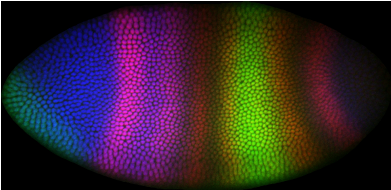
\includegraphics[height=0.35\textheight]{figures/Drosophila.png}
\vspace{0.5cm}
% %\captionof{figure}{first image}
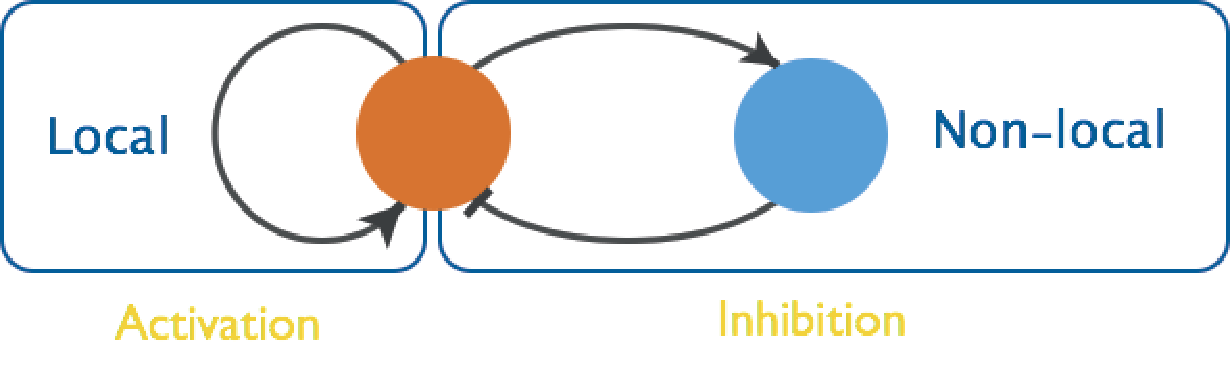
\includegraphics[height=0.35\textheight]{figures/turing.pdf}
% %\captionof{figure}{second image}

%Figure 1: Drosophila body segmentation genes. Blue stripes correspond... - Scientific Figure on ResearchGate. Available from: https://www.researchgate.net/figure/236739418_fig1_Figure-1-Drosophila-body-segmentation-genes-Blue-stripes-correspond-to-hunchback-green [accessed Jul 6, 2016]


}

\jframe{Example: Tissues change shape during animal development}{
% bio 2 , the most ≠ possible from the first
.
}


\jframe{Example : urban geography}{

\textit{Simple model of urban morphogenesis in~\cite{raimbault2014hybrid}}

\medskip

$\rightarrow$ local interactions captured by density feedback

$\rightarrow$ global position captured by network centrality feedback and accessibility to amenities

\medskip
{\centering
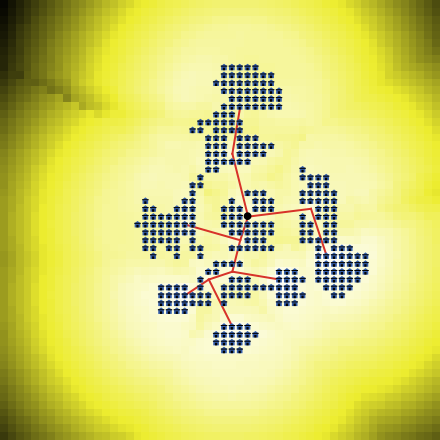
\includegraphics[width=0.5\textwidth]{figures/radiant}

}
}


\jframe{Example : psychology}{
Even though Morphogenesis has been sparsely used as a useful metaphor to understand different processes in various psychological fields, it is nonetheless a very powerful metaphor to conceptualize social change and of the subject within it and processes like the relation to evolution of human cultural behavior and learning.

 Neuroscience we have a plethora of morphogenetic phenomena related to the structure of the neural nets and “hardware” of the brain, and In Clinical psychology and psychopathology we have analogies to understand the emergence of psychical structures (Neurosis, Psychosis, etc) and the self-organization of relational forms (the self and the other), the formation of the symptom and of the transference-countertransference matrix. These structures form in early stages of development, but continue to repeat and influence behavior all throughout a subject’s life.
}


\jframe{Overview}{
% other numerous examples of fields/case of application
\begin{itemize}
\item \textbf{Biology}
\begin{itemize}
\item External phenotype morphogenesis (ant colony)~\cite{minter2012morphogenesis} \item Symbiosis of species~\cite{chapman1998morphogenesis}
\item Botany~\cite{}
\end{itemize}
\item \textbf{Social Sciences} : Archeology~\cite{renfrew1978trajectory}
\item \textbf{Epistemology} : \cite{gilbert2003morphogenesis}
\item \textbf{Artificial Intelligence} : From self-assembly to Morphogenetic Engineering. Synthetic Biology ?
\item \textbf{Geomorphology}
\item etc\ldots
\end{itemize}




}



%%%%%%%%%%%%%%%%%%
\section{Synthesis}


\jframe{Concepts}{
% common points and differences in concepts
\begin{itemize}
\item \textbf{Morphogenesis and Self-Organisation} : when does a system exhibit an architecture ? Insights from Morphogenetic Engineering~\cite{doursat2013review}. Architecture : the relation between the form and the function ?
\item \textbf{Scales, Units and Boundaries} From local interactions to global information flow (Holland's \emph{signal and boundaries}~\cite{holland2012signals}: morphogenesis as the development of Complex Adaptive Systems ?)
\item \textbf{Symmetry and Bifurcations} : on quantitative becoming qualitative. Ren{\'e} Thom's \emph{theory of catastrophes}~\cite{thom1974stabilite}
\end{itemize}

}




\jframe{Framework Proposition}{
% Generalisation based on the inclusion Self-organization > morphogenesis > autopoiesis > life.
% seems to include most of fields and ideas ?

% Processes of morphogenesis : local interaction vs information diffusion
.
}



\jframe{Perspectives}{
Systematize the framework : iterative construction

Algorithmic Literature Review and Text-mining


}


\jframe{Conclusion}{
.
}




%%%%%%%%%%%%%%%%%%%%%%%%%%%%%%%%
\begin{frame}[allowframebreaks]
\frametitle{References}
\bibliographystyle{apalike}
\bibliography{biblio}
\end{frame}
%%%%%%%%%%%%%%%%%%%%%%%%%%%%%%%%





\end{document}

